Tilting of the accelerator optical elements about the beam axis induces a non-zero average radial magnetic field, which causes an EDM-faking MDM precession. 

We have simulated the machine imperfection precession rate $\W_{MDM}$ for the frozen spin lattice depicted in Figure~\ref{fig:Lattice}. The lattice utilizes cylindrical E+B field spin rotators in the arc sections in order to effect the frozen spin condition. Imperfections were simulated via rotations of the E+B elements about the optical axis by normally-distributed angles $\Theta_{tilt}\sim N(0,10^{-4})$~rad. The standard deviation of $10^{-4}$~rad was chosen as an estimate of a practically-achievable element alignment error level. Analytical estimates~\cite{Senichev:FDM} show, that at this level, the machine imperfection $\W_{MDM}$ should be expected in the range of 50 to 100 rad/sec, assuming an $n=100$ element lattice.

\begin{figure}[h]\centering
	\includegraphics[width=\linewidth]{Figures/BNL}
	\caption{Frozen spin lattice with cylindrical E+B field spin rotators inserted into the arc sections.\label{fig:Lattice}}
\end{figure}

Simulation results are presented in Figure~\ref{fig:MDM_vs_tilt}. One can observe that at $\avg{\Theta_{tilt}}=10^{-4}$~rad the radial component of $\W_{MDM}$ is approximately 500~rad/sec. 
Since $\sigma[\avg{\Theta_{tilt}}]~=~\sigma[\Theta_{tilt}]/\sqrt{n} = 10^{-4}/\sqrt{100} = 10^{-5}$~rad. The dependence in Figure~\ref{fig:MDM_vs_tilt} is linear, hence the probability of observing $\W_{MDM}\le 50$~rad/sec is 68\%, $\W_{MDM}\le 100$~rad/sec is 95\%, and $50\le\W_{MDM}\le100$~rad/sec with a 27\% probability.

\begin{figure}[h]\centering
	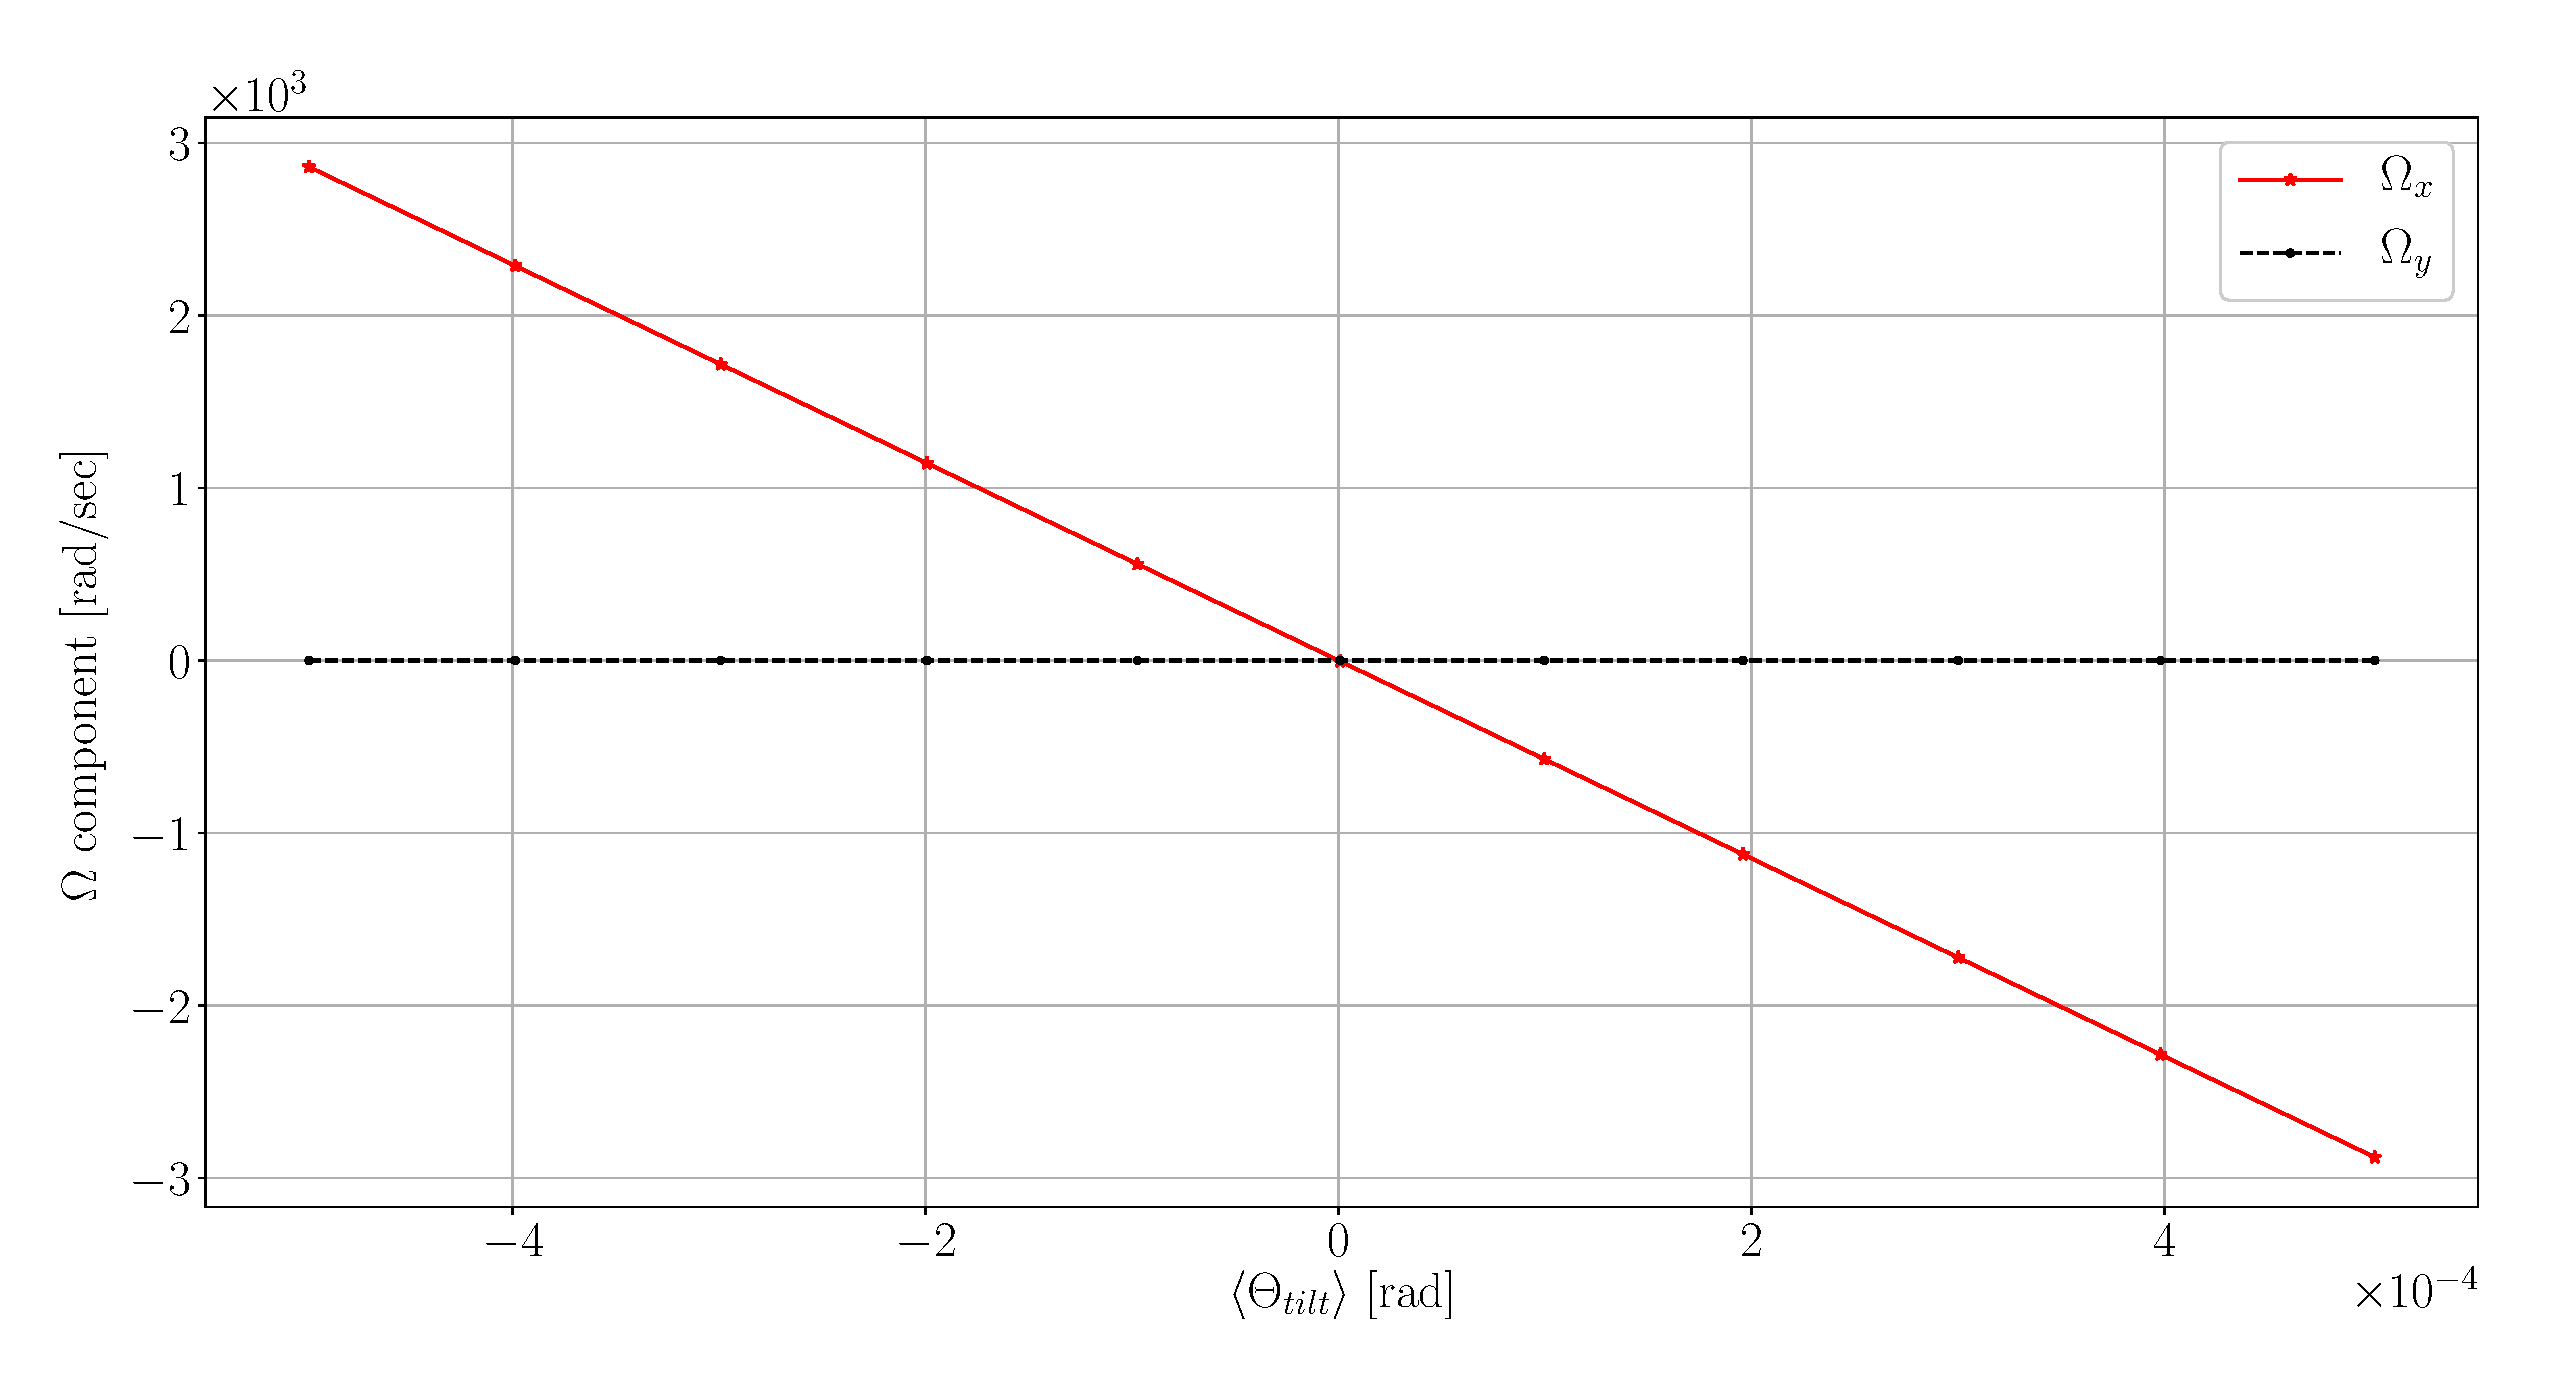
\includegraphics[width=\linewidth]{Figures/linearity_test_shifting_gauss_freq}
	\caption{Spin precession angular velocity components vs mean E+B element tilt angle.\label{fig:MDM_vs_tilt}}
\end{figure}